\documentclass[a4paper,12pt]{article}
\usepackage{amsmath}
\usepackage[utf8]{inputenc}  
\usepackage{graphicx}       
\usepackage{geometry}
\usepackage{parskip}
\usepackage{textcomp}
\usepackage{wrapfig}
\usepackage{caption}
\usepackage{listings}
\usepackage{xcolor}
\usepackage[inkscapelatex=false]{svg}
\usepackage[
backend=biber,
style=apa,
sorting=ynt
]{biblatex}

\addbibresource{sources.bib}


\definecolor{darkgreen}{rgb}{0.0, 0.5, 0.0}
\lstdefinelanguage{RAPID}{
  morekeywords={MODULE, PROC, VAR, CONST, IF, THEN, ELSE, WHILE, FOR, TO, ENDFOR, RETURN, TRUE, FALSE, PERS, TASK, ENDPROC, ENDIF, ENDWHILE, TEST, CASE, DEFAULT, ENDTEST, STOP, ERROR, TRAP, CONNECT, DISCONNECT, RAISE, EXIT, ENDTRAP, WITH, ISignalDI},
  sensitive=true,
  morecomment=[l]{!},       % Single-line comment
  morecomment=[s]{/*}{*/},   % Multi-line comment
  morestring=[b]{"}         % Strings wrapped in "
}

\lstdefinestyle{rapidstyle}{
  language=RAPID,
  basicstyle=\ttfamily\footnotesize,
  keywordstyle=\color{blue}\bfseries,
  stringstyle=\color{red},
  commentstyle=\color{darkgreen},
  numbers=left,
  numberstyle=\tiny,
  frame=single,
  backgroundcolor=\color{gray!10},
}

\lstset{style=rapidstyle}

\geometry{a4paper, margin=2.5cm} 

\begin{document}

\begin{titlepage}
    \centering
    \pagenumbering{gobble}
    \vfill
    
    \title{ABB RobotStudio, YuMi Application \& YuMi Challenge \\ \large TEL200 technical report\vspace{10cm}}
    \author{J\o rgen Asmundvaag \\ Ludvik H\o ibjerg-Aslaksen \\ Christopher Ljosland Strand}
    \date{March 2025}
    \maketitle
    \vfill
    \begin{figure}
        \includesvg[width=0.45\columnwidth]{NMBU_logo.svg}
    \end{figure}
    \vfill
\end{titlepage}

\section*{Abstract}
Jørgen Asmundvaag, Ludvik Høibjerg-Aslaksen, Christopher Ljosland Strand

ABB RobotStudio, YuMi Application \& YuMi Challenge, 10 pages

TEL200 technical report

Norwegian University of Life Sciences

Faculty of Science and Technology

March 2025

Instructor: Alireza David Anisi, Norwegian University of Life Sciences
\vspace{3em} % or try 2em for more space

This report presents two projects developed using the ABB YuMi IRB\textsuperscript{\textregistered} 1400 collaborative robot, conducted as part of the TEL200 course at NMBU. The aim was to explore both fundamental robotic operations and creative, open-ended problem-solving in a simulated and physical environment.

In the first task, the \textit{YuMi Application}, the robot was programmed to move three distinct geometric objects—a cube, cylinder, and prism—between designated slots on a grid. This application focused on precise manipulation using pose definitions, joint movements, and kinematic control. Safety functionality was implemented via an emergency stop button, integrated using smart components and RAPID trap routines.

In the second task, the \textit{YuMi Challenge}, we developed a semi-automated chess-playing system where the YuMi robot performed the Scholar's Mate opening against a human player. This task involved creating CAD models of chess pieces using 3D scanning, constructing a virtual chessboard in RobotStudio, and defining complex robot paths with collision avoidance and gripper adjustments.

Throughout both projects, we gained practical experience with RobotStudio, RAPID programming, and robotic simulation. The tasks provided insight into the capabilities and limitations of collaborative robots and demonstrated the importance of iterative testing, problem-solving, and system integration in robotics engineering.

\pagenumbering{arabic}

\newpage
\tableofcontents
\newpage

\iffalse
\section{Introduction}
Industrial robotics plays an increasingly vital role in modern manufacturing, increasing productivity, precision, and efficiency. ABB RobotStudio and the RAPID language provide a powerful platform for simulating and developing robotic operations in a virtual environment prior to physical implementation. This report presents two distinct tasks, each detailed in the sections below.

The first task called \textit{YuMi Application}, the goal of this task was to move three different shaped objects from their initial position to their designated final position. 

The second application is the \textit{YuMi challenge} where we were given a open-ended task to test the capabilities of the YuMi robot. Inspired by the famous 18th-century chess automaton \textit{The Mechanical Turk} \cite{mechanicalturk2025}, we decided to have the YuMi Robot play chess against us. Like \textit{The Mechanical Turk} the YuMi Robot is not autonomous and it uses pre-programmed moves to execute the Scholar's Mate. This  provides an insight into the functionality of the YuMi robot and it´s capabilities in performing precise tasks.
\fi

\section{Introduction}
Industrial robotics plays an increasingly vital role in modern manufacturing, increasing productivity, precision, and efficiency. ABB RobotStudio and the RAPID language provide a powerful platform for simulating and developing robotic operations in a virtual environment before implementation.

This project is part of the TEL200 course and focuses on working with the ABB YuMi robot using RobotStudio. The project is divided into three parts. 
In the first part, called the \textit{RS Basics}, we learned basic use of RobotStudio and RAPID programming.
The second part, called the \textit{YuMi Application}, involved moving three differently shaped objects between specific slots and back again.

In the third part, called the \textit{YuMi Challenge}, we were given a creative and open-ended task. We chose to make the YuMi robot play chess using pre-programmed moves. Inspired by the famous 18th-century chess automaton \textit{The Mechanical Turk} \parencite{mechanicalturk2025}, we decided to have the YuMi Robot play chess against us. Like \textit{The Mechanical Turk}, the YuMi Robot is not autonomous and the YuMi Robot followed a defined set of moves to execute the Scholar's Mate. This provides insight into the functionality of the YuMi robot and its capabilities in performing precise tasks.
\section{Method}
\subsection{Theory}
In this chapter, some important concepts are presented to help understand how a robotic arm moves.

\subsubsection{Poses}
The pose of an object describes its position and orientation relative to a known reference point. It can be mathematically represented using a homogeneous transformation matrix:

\[
T = 
\begin{bmatrix}
R & t \\
0 & 1
\end{bmatrix}
\]

- \( R \) represents orientation (rotation matrix).

- \( t \) represents position (translation vector).

\[
\begin{array}{c@{\hspace{2cm}}c}
\text{2D:} &
\text{3D:} \\
\begin{bmatrix}
r_{11} & r_{12} & x \\
r_{21} & r_{22} & y \\
0 & 0 & 1
\end{bmatrix}
&
\begin{bmatrix}
r_{11} & r_{12} & r_{13} & x \\
r_{21} & r_{22} & r_{23} & y \\
r_{31} & r_{32} & r_{33} & z \\
0 & 0 & 0 & 1
\end{bmatrix}
\end{array}
\]


\subsubsection{Path and Trajectory}
A \textit{path} defines how the robot moves from one pose to another, without specifying timing. A \textit{trajectory} includes timing information, determining how fast and when the robot passes through each point along the path.

\subsubsection{Joint space and Cartesian space}
Robot motion can be calculated in either \textit{joint space} or \textit{Cartesian space}:

- \textbf{Joint space} represents the robot's configuration using joint angles. It allows for simpler calculations but typically results in curved paths for the end-effector, which may be unsuitable for tasks requiring straight-line precision \parencite{corke2017}.

- \textbf{Cartesian space} plans motion based on the end-effector's position in space, enabling accurate, linear movements. However, it involves more complex computations and can lead to high joint velocities, especially near singularities.\parencite{corke2017}.

\subsubsection{Singularities}
Singularities are specific configurations where the robot loses some degrees of freedom, which can cause instability, unpredictable motion, or high joint speeds \parencite{corke2017}. Robots with more joints, like the ABB YuMi which has 7 axes, are considered over-actuated. This means they have more degrees of freedom than strictly necessary to position their end-effector, allowing them to avoid singularities more easily. As a result, YuMi can find alternative joint configurations to reach a target pose, making it more flexible and suitable for complex or constrained tasks.

\subsubsection{ABB YuMi IRB 1400}
The ABB YuMi IRB 1400 is a dual-arm, 7-axis collaborative robot designed for high-precision tasks in collaboration with humans. Its redundant kinematic structure enables advanced motion planning and increased flexibility, which makes it useful for tasks where the robot needs to avoid obstacles and handle objects with care.

\subsection{YuMi Application}
The workstation contains a cube, cylinder, and prism, each with two slots arranged in a 3x3 grid. The task is to move the objects between slot 1 and 3 and return to the start upon button press. No changes to the object models were needed, as they were already implemented.

\subsubsection{Creating the Paths and Targets}
The grid is defined from the global coordinate system, with 100 mm between each slot center. Columns represent slot positions (x-axis), and rows define object types (y-axis). The robot moves each object from column 1 to 3 or vice versa.

Since the gripper aligns its local coordinate system with the object's, all target frames must be rotated 180° around the x- or y-axis. For the cube, we define an approach point above and a grasp point below to avoid collisions. The cylinder follows a similar setup but requires precise centering. The prism requires an additional 90° rotation to allow gripping it by its corner and side for a secure hold.


\subsubsection{Code Structure and Timings}
At the beginning of the RAPID code, all targets and the variables used to track which side the object currently is on, along with two key variables: \textit{speed} and \textit{precision}, controlling speed and accuracy.

The main logic is inside a \texttt{while} loop that continuously checks button inputs. Depending on which button is pressed, the code calls specific functions to move the corresponding object accordingly.

\iffalse
For example, when the green button with the signal \textit{di\_cube} is pressed, the program first determines the direction the cube should move, subsequently calling either the \textit{cube\_left\_right} or \textit{cube\_right\_left} functions. These functions guide the robot to an upper target point, open the gripper, move down to grasp the object, close the gripper, move back up, transfer to the opposite side, descend again, release the object, and finally return to the starting position. The same logic and procedure is similar for the cylinder and prism.
\fi

When the green button \textit{di\_cube} is activated, the program evaluates the cube’s current position and calls either \textit{cube\_left\_right} or \textit{cube\_right\_left} to execute the appropriate path. Each function moves the robot to a predefined approach point, opens the gripper, descends to the grasping position, closes the gripper, lifts the object, transfers it to the target slot, lowers it, releases the object, and returns to the home position. The same control logic is applied to both the cylinder and prism, with minor variations for the different shapes of the objects.

\subsubsection{Creating the Mechanism of the Emergency Button}
\iffalse
\begin{wrapfigure}{r}{0.25\textwidth}
  \label{fig:create_joint}
  \centering
  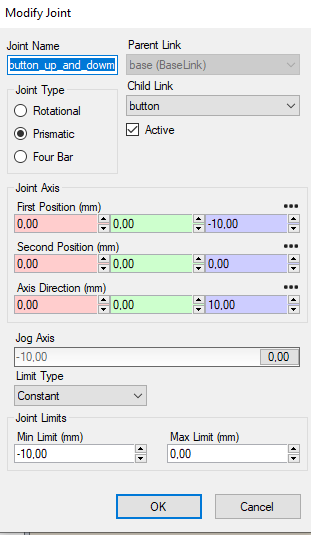
\includegraphics[width=0.2\textwidth]{create_joint.png}
  \caption{Create joint}
\end{wrapfigure}
\fi
The first step towards animating the button is to create a mechanism. This can be done by pressing the create mechanism button under the modeling tab.

The second step is to create links and joints. First create the links with the e-stop base as the baselink, and the e-stop button as childlink. Then to create joints choose prismatic as the joint type. Set the min limit to -10 mm and the max limit to 0 mm.

\subsubsection{Simulating The Emergency Button}
The emergency stop button needs to stop all movements when pressed and when let go, start all movement. To achieve this a trap routine must be used, this is due to its ability to interrupt a command at any moment. The trap routine can be created using the syntax below:
\begin{lstlisting}
    TRAP EmergencyStop
        StopMove;
        WaitUntil di_EmergencySituation = 0;
        StartMove;
    ENDTRAP
\end{lstlisting}
The code block below needs to be inside module: 
\begin{lstlisting}
VAR intnum stop_emer; ! interrupt number datatype
\end{lstlisting}
The code block below needs to be inside main:
\begin{lstlisting}
    ! Connects the intnum with the trap routine EmergencyStop
    CONNECT stop_emer WITH EmergencyStop;
    ! Handles checking whether the emergency stop button is pressed
    ISignalDI di_EmergencySituation, high, stop_emer;
\end{lstlisting}
When a pose mover receives a high signal to its Execute it will move the mechanism to that pose. Connecting the input to a NOT logic gate then to a pose mover allows it to be in that pose when the input is low. Then connecting the input directly to a different pose mover allows the mechanism to alternate between two different poses. The input also needs to be connected to the output for later use in station logic. See figure~\ref{fig:smart_component_emer} for a picture of the smart component.

\begin{wrapfigure}{r}{0.43\textwidth}
    \centering
    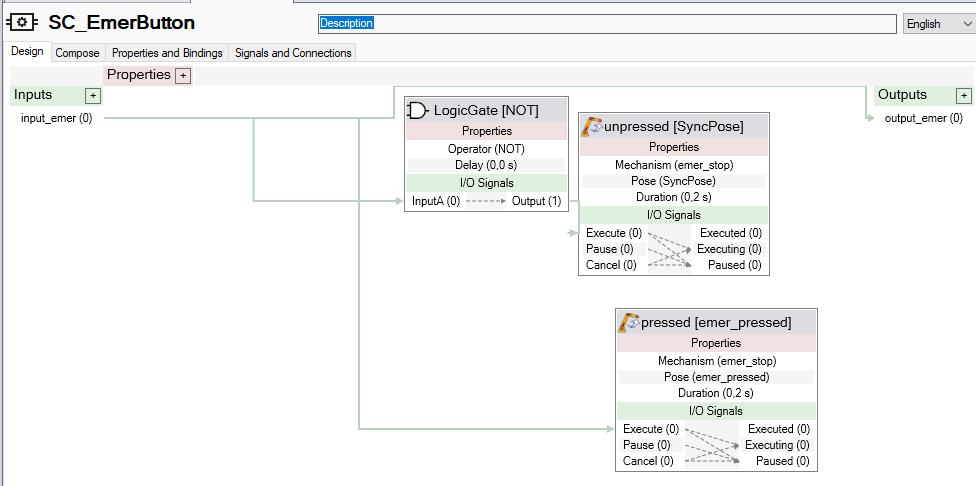
\includegraphics[width=1\linewidth]{SC_emer_button.png}
    \captionsetup{font=scriptsize}
    \captionof{figure}{Smart component of the emergency button}
    \label{fig:smart_component_emer}
\end{wrapfigure}

To connect the functionality of the emergency button to the simulated movement a few connections in station logic is required. First create a signal named do\_EmergencySituation with access level all. Then connect it to the input of the emergency button smart component. Finally connect the output of the emergency button smart component to di\_EmergencySituation.

\subsection{YuMi Challenge}
\subsubsection{CAD geometry}
To be able to get accurate placements of the chess pieces, we modeled a chessboard using the rectangle surface geometry option in RobotStudio. Using this we created a 25x25mm square surface, and assembled a chessboard from 64 of these rectangles. We centered the board axis to align with the target of the \textit{wobj0}, to simplify our setup process. We also aligned the border of the board 200 mm from the \textit{wobj0} target.

To create the CAD geometry, we used a 3D scanner borrowed from Eiklab to generate a 3D model of each chess piece. These files were then imported into Fusion360, where we inserted the mesh, rotated each piece to ensure proper alignment, and exported them as .sat files for use in RobotStudio.

When all .sat files were finished, we imported them into RobotStudio using the import CAD geometry button. After importing the pieces we positioned them at their correct places using trial and error, and then used the duplicate function to place identical pieces on every square.

\subsubsection{Creating the paths and targets}
\label{sec:Challenge_paths_targets}
When creating the paths, we based the targets on the chess moves from table~\ref{tab:chess_moves}.

\begin{table}[h] %Scholar's mate moves
    \centering
    \begin{tabular}{c l l}
        \hline
        Move & White & Black \\
        \hline
        1. & e4 & e5 \\
        2. & Dh5 & Sc6 \\
        3. & Lc4 & Sf6?? \\
        4. & Dxf7 & (checkmate) \\
        \hline
    \end{tabular}
    \caption{Scholar's Mate}
    \label{tab:chess_moves}
\end{table}
To make the YuMi Robot's moves as smooth as possible it is important to have two targets above the desired destination. One that is about 5 mm above the chess piece and one that is higher in the range 25-50 mm above the piece. This allows the YuMi Robot to move smoothly between each target. Due to the 3D-scans being somewhat inaccurate the distances specified may need some adustments depending on the piece and quality of the model.

To simplify the paths the YuMi Robot returns to a set point after picking up or placing a piece. This point is centered above the queen with a 25 mm offset towards the YuMi Robot. 

After the paths have been created it is important to note that a fully extended gripper would collide with pieces surrounding the piece to be picked up. To solve this the RAPID command \textit{g\_MoveTo value;} was used. This command extends the gripper to the specified value, allowing the gripper to easily slide between the pieces. The gripper was extended to 7 mm for the large pieces and 8 mm for pawns.

After finishing moving all the chess pieces, the YuMi robot moves its arm in a celebratory movement. When running the celebration, the arm has to move quite far up, so to achieve this, a helping point has to be used to avoid collisions.

\subsubsection{Code structure and timings}
The top part of the code consists of all the targets and three variables called speed, precision and timing. The variables control how fast the YuMi Robot moves, how precise and seconds between each  chess move. The main body of the RAPID code consists of while loop that is constantly true allowing the code to run in a loop, within the while loop the code has several if statements that check whether the buttons have been pressed or not. 

The green button \textit{di\_cube} when pressed runs move 1 from table~\ref{tab:chess_moves}. When it is pressed a second time it runs move 2 and so on. After all moves are run it resets to move 1. The second blue button \textit{di\_cylinder} runs all moves with timing delay specified in the code by a variable. The third red button \textit{di\_prism} runs the celebration described in section \ref{sec:Challenge_paths_targets}. The fourth yellow button \textit{di\_home} returns the YuMi Robot to its start position.

The final button is an emergency stop button called \textit{di\_EmergencySituation} this button when pressed runs a trap routine that stops the YuMi Robot mid path, and when let go it continues the operation. One of the main advantages of using a trap routine is that it can interrupt any movement and immediately issue commands - something that would not be achievable with if statements.

\subsubsection{Physical development}
\begin{figure}[h!]
    \centering
    \includegraphics[width=0.25\linewidth]{Frame 131.png}
    \caption{Chessboard }
    \label{fig:enter-label}
\end{figure}
To get a chess board with the same size as the one in the simulation, we had to create a custom board. This was done using Figma where we created an A4 frame with 25x25mm squares, and a cross marking the center of each square. This then got exported as a PDF and was printed out.



\section{Results}
\subsection{YuMi Application}
For the YuMi Application task, we found several results during our work on the robot. By applying the knowledge on poses and joints from the lectures, we managed to move all the geometric shapes to the opposite side and back to their starting position. 

We encountered some issues during our implementation of the YuMi Application. Our earliest version had some issues with table clearance, and when moving the cylinder we encountered an error that said a joint was moving in the wrong direction.

\subsection{YuMi Challenge}
\label{sec:YuMi_challenge_results}
The YuMi challenge did not present significant issues regarding configurations; however, we encountered challenges related to the space between chess pieces and achieving proper grip on certain pieces. Chess pieces would also sometimes get stuck to the gripper, resulting in inaccurate placement or them tipping over. At the beginning we also had some issues where the gripper would bump pieces on its way back. In the end we managed to successfully perform a Scholar's Mate using the YuMi Robot.

\section{Discussion}
\subsection{YuMi Application}
An area where we could have improved would be the paths that the YuMi is following. We have seen improvements in every version of our program, and the paths that ended up being used was the simplest and most linear we managed to create. An area for improvement would be the clearance between the gripper and obstacles. Even though the robot is moving clear of any objects and collisions, some positions on the path could use more clearance. A final improvement would be to use the built in reverse path, instead of creating our own path to move the objects back.

Our earliest issues with clearance was solved by having the gripper move towards the pieces from targets located higher up from the table. The issue with a joint moving in the wrong direction was solved by using the signal analyzer to see if the joint was close to 180 degrees, and changing configurations with the box include turns checked.
\subsection{YuMi Challenge}
To achieve a Scholar's Mate all the moves were hardcoded with paths and targets, since anything more involved would be beyond the scope of TEL200. As mentioned in section \ref{sec:YuMi_challenge_results} we encountered several issues during implementation. 

To solve our issue with gripper bumping pieces on its way pick up a piece. We used the RAPID command g\_MoveTo, this allowed us to open the gripper partially, and let the gripper easily slide between chess pieces. We also had some issues with the gripper bumping pieces on its way back after placing a piece. This was solved by placing a target slightly above the piece to be grabbed or placed. Then place a target far enough above such that the gripper would clear the pieces before moving back.

During our implementation, we encountered an issue where some pieces, especially the queen and bishop would get stuck to the gripper resulting in them being placed at the wrong spot or tipping over. To fix this, we placed a piece of tape over the gripper where the pieces was getting stuck. After placing the tape everything worked as intended.

Before deciding to define the moves as predefined paths, we explored the possibility of using the buttons to control forward/backward, left/right, and pick up/place actions. This approach would emulate a game controller, allowing the user to play any move on the board manually. This would have taken more time to implement than we had available for the challenge, and the precision could be hard to maintain over a longer game, as the pieces tend to move when placed.

If we were to do this project again, we would implement a coordinate system of all targets on the chess board, to simplify the manipulation of the pieces' positions.

\section{Conclusion}
The ABB YuMi 1400 cobot is powerful and versatile. Throughout the projects, we observed both its capabilities and its limitations. Having the opportunity to develop in RobotStudio, test our code on the robot, debug, and return to RobotStudio enabled us to quickly patch bugs, test new approaches, and refine our code.


For the YuMi application, we applied theoretical concepts from the lectures to gain an understanding of pose, movement and robotic system development.

For the YuMi Challenge, having the freedom to choose our task, provided another perspective on working with cobots and allowed us to explore their practical applications.

During this project, we have thoroughly tested and experienced both the possibilities and limits of collaborative robots. The YuMi application allowed us to practice and gain foundational skills in RobotStudio and RAPID development. Overall, this project gave us a solid learning experience and made us much more comfortable using RobotStudio, RAPID programming, and working with collaborative robots.
\nocite{*} % outputs everything without them being cited in the text
\printbibliography
\end{document}
